\documentclass[12pt]{article}
\usepackage[english]{babel}
\usepackage[utf8x]{inputenc}
\usepackage{amsmath}
\usepackage{graphicx}
\usepackage{subcaption}
\usepackage[export]{adjustbox}
\PassOptionsToPackage{hyphens}{url}
\usepackage{hyperref}

\graphicspath{ {../../Images/} }

\usepackage{xcolor}

\definecolor{codegreen}{rgb}{0,0.6,0}
\definecolor{codegray}{rgb}{0.5,0.5,0.5}
\definecolor{codepurple}{rgb}{0.58,0,0.82}
\definecolor{backcolour}{rgb}{0.95,0.95,0.92}

\hypersetup{
    colorlinks=true,
    linkcolor=blue,
    filecolor=magenta,      
    urlcolor=blue,
}
\usepackage{listings}
\lstdefinestyle{mystyle}{
    backgroundcolor=\color{backcolour},   
    commentstyle=\color{codegreen},
    keywordstyle=\color{magenta},
    numberstyle=\tiny\color{codegray},
    stringstyle=\color{codepurple},
    basicstyle=\ttfamily\footnotesize,
    breakatwhitespace=false,         
    breaklines=true,                 
    captionpos=b,                    
    keepspaces=true,                 
    numbers=left,                    
    numbersep=5pt,                  
    showspaces=false,                
    showstringspaces=false,
    showtabs=false,                  
    tabsize=2
}
\lstset{style=mystyle}

\begin{document}

\begin{titlepage}

\newcommand{\HRule}{\rule{\linewidth}{0.5mm}} 

\center
-------------------------------------------------------------------------------------

\textsc{\LARGE Politenico di Milano}\\[1cm]
\textsc{\Large Dipartimento Elettronica, Informazione e Bioingegneria}\\[0.5cm] 
\textsc{\large Homework IoT Project}\\[0.5cm] 

%----------------------------------------------------------------------------------------
%	TITLE SECTION
%----------------------------------------------------------------------------------------

\HRule \\[0.4cm]
{ \huge \bfseries From Device to Platform}\\[0.4cm]
\HRule \\[1.5cm]
 
%----------------------------------------------------------------------------------------
%	AUTHOR SECTION
%----------------------------------------------------------------------------------------

\begin{minipage}{0.4\textwidth}
	\begin{flushleft} \large
		\emph{Author:}\\
		Francesco \textsc{Monti}\\
		Matr: 919755 
	\end{flushleft}
\end{minipage}
~
\begin{minipage}{0.4\textwidth}
	\begin{flushright} \large
		\emph{Supervisor:} \\
		Dr. Edoardo \textsc{Longo}\\
		Dr. Matteo \textsc{Cesana}
	\end{flushright}
\end{minipage}\\[1.5cm]


%----------------------------------------------------------------------------------------
%	DATE SECTION
%----------------------------------------------------------------------------------------

{\large \today}\\[2cm] 

%----------------------------------------------------------------------------------------
%	LOGO SECTION
%----------------------------------------------------------------------------------------

\begin{figure}[h]
	\begin{subfigure}{0.5\textwidth}
		
\includegraphics[width=150pt, left]{Logo_Politecnico_Milano.png}
	\end{subfigure} 
	\begin{subfigure}{0.5\textwidth}
		
\includegraphics[width=100pt, right]{Ant_Lab_Logo.png}
	\end{subfigure}
\end{figure} 
 
%----------------------------------------------------------------------------------------

\vfill

\end{titlepage}
\begin{abstract}
This document offers some comments for the fifth activity for the course ``Internet of Things'', Academic Year 2019/2020. \\
This document has been also uploaded on the following GitHub repository: \url{https://github.com/Framonti/IoT_Projects}\\
The results were uploaded to the following TeamSpeak channel: \url{https://thingspeak.com/channels/1070054}
\end{abstract}
\subsection{Comments on Implementation}

\begin{itemize}
\item Instead of using a fixed topic (so, a string), the motes sends a TopicID (1 for mote2, 2 for mote3). The final topic processing is left to Node-RED.
\item The motes send messages as JSON strings, in the form \{``Value'': \textit{value}, ``TopicID'': \textit{TopicID}\}. However, due to compatibility issues with Cooja, what is received is slightly different (see \ref{fig:messages}). A function in Node-RED takes care of this problem, and restores the original string. 
\item Since ThingSpeak limits the number of receivable samples in a time interval, we introduced a Rate Limiter in Node-RED (1 sample/minute).
\item The random generation of values is delegated to the TinyOS component RandomC.
\item We generated and plotted more or less 30 samples smaller than 70.
\end{itemize}
\begin{figure}[h]
	\centering
	\captionsetup{justification=centering}
	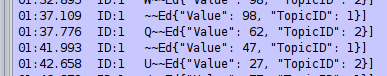
\includegraphics[width=\textwidth]{cooja-messages.png}	
	\caption{Messages Received by Cooja}
	\label{fig:messages}
\end{figure}

\end{document}